\section{Introduction}
\label{sec:introduction}

Address translation is a first-order performance concern in modern GPU workloads~\cite{power_x86}.
As applications move toward larger, irregular memory footprints such as sparse graph
traversal, scientific stencils, and machine learning inference over large embedding tables,
the GPU L2 TLB becomes a sustained bottleneck \cite{ganguly_interplay, shin_irregular}.
Prior work has approached this problem almost exclusively from an access-pattern perspective,
predicting which virtual pages will be needed next and prefetching their translations
before the demand miss occurs~\cite{latpc,valkyrie, mosaic, snake_prefetch}.
This framing implicitly treats each TLB miss as a cold event requiring a fresh page walk,
but many TLB misses are not cold at all. A \emph{dead-entry TLB miss} occurs when a virtual page whose translation is still valid
is evicted from the TLB and then re-accessed before the working set rotates again.
The page walk is not cold; it is redundant.
The entry was alive, was discarded by LRU replacement, and is now being reconstructed
at full page-walk cost.
Measuring this phenomenon across 24 GPU workloads reveals that dead-entry misses are
pervasive: in the most TLB-sensitive applications, over 99\% of all L2 TLB misses
carry an eviction-history signature.

\begin{figure}[t]
  \centering
  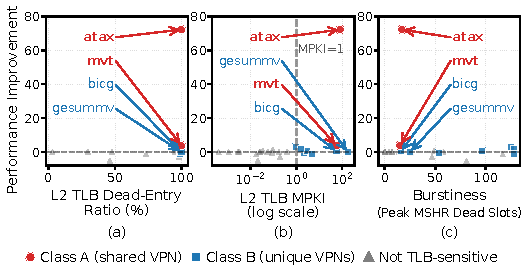
\includegraphics[width=\figwidth]{figs/fig01_teaser.pdf}
  \caption{Performance improvement (IPC) from eliminating dead-entry re-walks against three candidate predictors: (a)~DE ratio, (b)~MPKI, and (c)~MSHR burstiness, for all 24 workloads.}
  \label{fig:teaser}
\end{figure}

Yet the performance consequences of dead-entry misses are not uniform, and
Figure~\ref{fig:teaser} shows why simple miss statistics fail to explain the divergence.
Each plot shows the performance improvement from eliminating dead-entry re-walks against a different
candidate predictor for all 24 workloads.
Figure~\ref{fig:teaser}(a) shows that dead-entry ratio has no predictive power: all TLB-sensitive workloads
cluster near 99\% dead-entry ratio, yet their performance improvement ranges from near zero to $72\%$.
Figure~\ref{fig:teaser}(b) shows that MPKI is necessary but not sufficient: workloads with large IPC improvements
and workloads with near-zero improvements remain indistinguishable at similar MPKI levels.
Figure~\ref{fig:teaser}(c) reveals the discriminator: burstiness, measuring how many pending translation requests
are collectively served by a single page walk; workloads with high burstiness achieve large performance
improvements, while those with near-zero burstiness achieve near-zero improvements.

In some workloads, all threads in a warp reference the same memory page, so a single TLB
eviction stalls many warps simultaneously waiting for one translation to return.
Eliminating that redundant re-walk unblocks all of them at once, producing large performance
improvements and high observed burstiness.
In other workloads, each thread accesses a distinct page from a working set that exceeds
TLB capacity.
Evictions are driven by the sheer size of the working set, and no replacement-level
mechanism can eliminate them because the TLB simply cannot hold all required translations
at once.
These two root causes lead to opposite outcomes under any dead-entry protection mechanism,
and we characterize and validate both across all 24 workloads in Section~\ref{sec:characterization}.

Building on this characterization, we design \emph{DEPOT} (Dead-Entry PrOTection),
a lightweight hardware mechanism that targets the first type of workload.
DEPOT uses a small Bloom filter to track recently evicted TLB entries and temporarily
protects re-installed entries from being displaced again, preventing the same redundant
re-walks from compounding.
The mechanism requires approximately 3.5\,KB of storage, introduces no prediction logic,
and falls back gracefully to standard LRU replacement for workloads where it provides
no benefit.
DEPOT also composes well with LatPC~\cite{latpc}, the state-of-the-art TLB prefetching
and compaction mechanism, because the two techniques address fundamentally different
sources of misses.
LatPC reduces misses through stride prediction and entry compaction; DEPOT prevents
recently used pages from being discarded prematurely.
Together they outperform either mechanism alone by 2 to 7\% on TLB-sensitive workloads
at negligible additional hardware cost.

In this paper, we make the following contributions.
\begin{itemize}
  \item \textbf{Eviction-history characterization.}
    We measure GPU L2 TLB misses by eviction history across 24 workloads,
    establishing dead-entry re-walks as a prevalent, structurally distinct miss class.
  \item \textbf{Two-class taxonomy.}
    We identify two root causes among TLB-sensitive workloads,
    interference-driven misses where multiple warps share the same virtual page,
    and capacity-driven misses where the working set exceeds TLB reach,
    and validate the taxonomy using 2\,MB huge page experiments.
  \item \textbf{DEPOT mechanism and composition.}
    We design DEPOT (Dead-Entry PrOTection), a Bloom-filter mechanism
    (1\,KB filter, 3.5\,KB total)
    achieving up to 72\% performance improvement on interference-driven workloads and
    2 to 7\% additive improvement on top of LatPC~\cite{latpc},
    the state-of-the-art TLB prefetching and compaction mechanism.
\end{itemize}